\section{Middleware}

L'obiettivo del nostro progetto è stato quindi quello di realizzare un servizio web per fornire statistiche sui match NBA e provare a predirne i risultati. Come anticipato, abbiamo esteso questa idea creando un'applicazione web (analizzata in seguito) che permettesse non solo di prevedere l'esito di un match NBA, ma anche di fornire tutte le informazioni necessarie per valutare personalmente quale squadra avesse maggiori probabilità di vincere, includendo anche le quote offerte dai bookmakers. In pratica, il nostro progetto si è avvicinato alla realizzazione di un sito di scommesse con l'aggiunta di informazioni e previsioni sui match, ovviamente limitato al contesto NBA.

Per realizzare questa applicazione web, abbiamo avuto bisogno di due tipi di informazioni principali:
\begin{itemize}
    \item dati statistici sulle partite, sulle squadre e sui giocatori della NBA;
    \item informazioni sulle quote delle scommesse head-to-head e spread.
\end{itemize}

\subsection{Swagger OAS 3.0}

Abbiamo deciso di implementare i nostri middleware come REST API server, essendo uno standard affermato per la creazione di servizi web che offre benefici come flessibilità, scalabilità e facilità di manutenzione. Per implementare e documentare le nostre API in modo efficiente, abbiamo scelto di utilizzare l'Open API Specification 3.0 (OAS 3.0).

La specifica OAS 3.0 ci ha permesso di descrivere in dettaglio tutti gli endpoint disponibili, inclusi i parametri, le risposte (sia di successo che di errore) e i tipi di oggetti restituiti, con esempi dettagliati. Abbiamo utilizzato i servizi offerti da \href{https://editor.swagger.io/}{Swagger Editor} per generare automaticamente un'interfaccia utente che ci ha permesso di testare le nostre API con facilità, inizialmente basandoci solo sulla specifica testuale e ottenendo risposte fittizie, e infine utilizzando il progetto completo per ottenere risposte reali basate sulla logica di backend presente dietro ciascuno degli endpoint.

Questo approccio ci ha permesso di facilitare notevolmente lo sviluppo e la coordinazione tra i membri del team: è stato sufficiente definire la specifica testuale per permettere a chi sviluppava l'applicazione web e a chi implementava i middleware di lavorare in modo indipendente e parallelo, basandosi semplicemente sulla specifica OAS definita in precedenza. Inoltre, Swagger ci ha permesso di generare gli scheletri dei REST API server in modo automatizzato, prendendo in input solamente la specifica testuale in formato YAML. Questo ci ha dato un enorme vantaggio sia iniziale, per realizzare il progetto senza partire da zero, sia in termini di estensibilità futura. Infatti, per aggiungere nuovi endpoint, possiamo farli generare dallo stesso servizio e copiare nel nostro progetto solo le parti "nuove", con uno sforzo di implementazione minimo.

\begin{figure}[H]
    \centering
    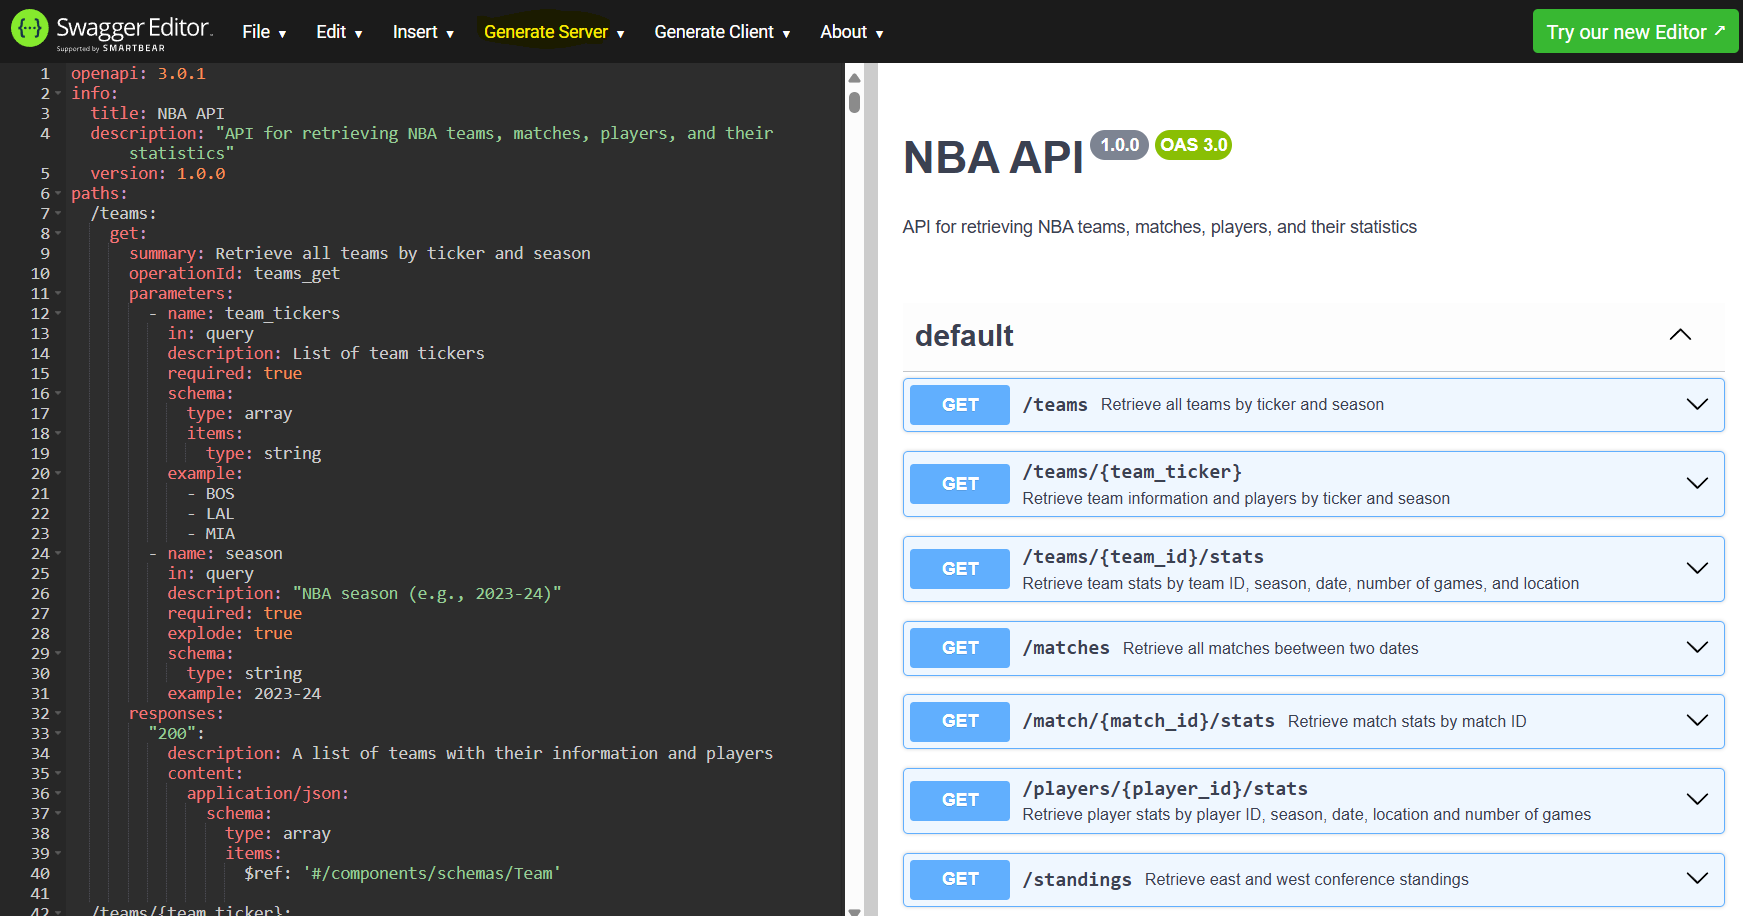
\includegraphics[width=0.75\textwidth]{img/swagger_ui.png}
    \caption{Interfaccia utente Swagger UI per testing e generazione server}
\end{figure}

\subsection{Bet API}

Partiamo dall'analisi della \texttt{bet\_api}, ovvero del servizio che permette alla \texttt{web app} di ottenere tutte le informazioni necessarie relative alle quote delle partite. Alla base di questa API è presente un'ulteriore API, che analizza tutti i siti dei bookmakers di varie regioni del mondo e restituisce le quote di ogni partita, relative a diversi mercati: \href{https://the-odds-api.com/}{The Odds API}.

Il concetto di middleware entra in gioco qui: avremmo potuto utilizzare direttamente l'API già esistente per ottenere tutte le informazioni di nostro interesse, ma così facendo abbiamo potuto semplificare gli endpoint, limitandoli alle sole informazioni di nostro interesse e richiedendo solo i parametri di input strettamente necessari. Inoltre, abbiamo centralizzato la gestione della sicurezza, sollevando la web app dal memorizzare e inviare ogni volta la \texttt{API key} per autenticarsi presso il servizio esterno.

\texttt{The Odds API} fornisce le quote non solo per la NBA, ma per qualsiasi sport presente su un sito di scommesse. Questo ci ha permesso di estendere ulteriormente le funzionalità della nostra applicazione e di realizzare di conseguenza il middleware \texttt{bet\_api}. Abbiamo scelto di strutturare gli endpoint in modo da supportare qualsiasi tipo di sport, senza limitarci alla sola NBA di nostro interesse iniziale. Questo comporta un minimo overhead in termini di complessità, ma offre grande flessibilità.

In questo modo, la nostra web app sarà in grado, in sviluppi futuri, di supportare e visualizzare le quote di qualsiasi sport presente su un sito di scommesse, sempre però limitate ai due mercati principali head-to-head e spread, che sono comuni alla maggior parte degli sport.

\subsubsection{Endpoint}

Di seguito vengono presentati gli endpoint disponibili:
\begin{itemize}
    \item \texttt{/sports/getSportGroups}\\
    Restituisce l'elenco di tutti i gruppi di sport disponibili. Questo endpoint supporta un parametro opzionale: \texttt{all}, che se impostato a \texttt{true} restituisce sia i gruppi sportivi in stagione (con partite attualmente in corso) che quelli fuori stagione. La risposta di successo, con codice 200, contiene un elenco di tutti i gruppi sportivi disponibili.
    \item \texttt{/sports/getSports}\\
    Restituisce l'elenco di tutti gli sport disponibili. Questo endpoint supporta due parametri opzionali: \texttt{groupName}, che consente di filtrare gli sport per nome del gruppo, e \texttt{all}, che se impostato a \texttt{true} restituisce sia gli sport in stagione che quelli fuori stagione. La risposta di successo, con codice 200, contiene un elenco di tutti le chiavi identificative degli sport disponibili.
    \item \texttt{/sports/getSportEvents}\\
    Restituisce l'elenco di tutti gli eventi disponibili per uno sport specifico. È necessario specificare il parametro obbligatorio \texttt{sportKey}, che indica la chiave dello sport degli eventi. Sono supportati due parametri opzionali: \texttt{commenceTimeFrom} e \texttt{commenceTimeTo}, che permettono di filtrare gli eventi in base al loro orario di inizio e di fine. La risposta di successo, con codice 200, contiene un elenco di tutti gli eventi disponibili.
    \item \texttt{/odds/head2head}\\
    Restituisce le migliori quote head-to-head per un evento specifico. È necessario specificare i parametri obbligatori \texttt{eventId} e \texttt{sportKey}, che indicano rispettivamente l'ID dell'evento e la chiave dello sport dell'evento. È disponibile un parametro opzionale \texttt{regions}, che consente di specificare la regione per ottenere le quote. La risposta di successo, con codice 200, contiene due elenchi delle quote head-to-head, ciascuno ordinato dalla quota più alta, uno relativo alla squadra di casa vincente e uno per quella in trasferta.
    \item \texttt{/odds/spreads}\\
    Restituisce le migliori quote head-to-head con handicap per un evento specifico. È necessario specificare i parametri obbligatori \texttt{eventId} e \texttt{sportKey}, che indicano rispettivamente l'ID dell'evento e la chiave dello sport dell'evento. È disponibile un parametro opzionale \texttt{regions}, che consente di specificare la regione per ottenere le quote. La risposta di successo, con codice 200, contiene due elenchi delle quote head-to-head con handicap, ciascuno ordinato dalla quota più alta, uno relativo alla squadra di casa vincente e uno per quella in trasferta.
\end{itemize}


\noindent Per ciascuno degli endpoint presentati sopra, sono previste risposte con codice 201 nel caso in cui non ci siano quote, eventi o sport da restituire, con codice di errore 400 per richieste errate e 500 per errori interni del server.

Da notare come, oltre al supporto per tutti gli sport grazie al parametro chiave \texttt{sportKey} (che avremmo potuto omettere inserendo sempre la chiave relativa all'NBA), vi è anche una logica per la restituzione delle quote per ogni match, ordinate dalla più vantaggiosa per l'utente, prendendo in considerazione tutti i siti di scommesse disponibili. In questo modo, tramite la web app, l'utente può avere una visione completa delle quote disponibili per ogni match e scegliere quella che ritiene più conveniente basandosi sui siti di scommesse sui quali ha un conto aperto.

Inoltre, abbiamo reso disponibili per l'utente i link ai vari siti di scommesse, in modo da facilitarne l'accesso e il controllo della quota mostrata. Per ottenere questa informazione, non disponibile direttamente da \texttt{The Odds API}, abbiamo effettuato dello scraping direttamente sul web, basandoci sul nome del sito fornito appunto dal servizio esterno.\\

\noindent \textbf{Nota}: Il file \href{run:../documents/bet_oas.yaml}{bet\_oas.yaml} presenta la specifica Open API 3.0 completa, utilizzata per generare il server iniziale.


\subsubsection{Dettagli implementativi}
A livello implementativo, è stato usato Spring Boot per costruire il middleware, sfruttando la potenza delle sue annotazioni per ottenere un codice altamente strutturato, pulito e flessibile. 

Inoltre, è importante sottolineare l'implementazione dell'autenticazione verso \texttt{The Odds API} tramite \texttt{API Key}. Abbiamo sfruttato il concetto di \textit{Interceptor} di Spring, un componente che si interpone prima di ogni \textit{HttpRequest} e tramite il quale è possibile modificare i parametri e l'header della richiesta. Questo ci ha permesso di omettere sia l'url base della \texttt{Odds API} sia la \texttt{API Key} in ogni richiesta, poiché queste informazioni sono state salvate nel \textit{context} dell'applicazione e aggiunte automaticamente ad ogni richiesta in uscita.\\
Quindi, in caso di aggiornamenti dell'URL o di rinnovo dell'\texttt{API Key}, sarà sufficiente modificare solo il file di consigurazioni con le suddette informazioni, senza dover cercare e modificare ogni singola chiamata, portando grandi vantaggi in termini di manutenibilità.


\subsubsection{Quote storiche}
Il piano gratuito di \texttt{The Odds API} non ci ha permesso purtroppo di ottenere dati su eventi e quote storiche (già passate). Questo ci ha posto dei limiti nelle ultime fasi di sviluppo poiché, essendo terminata la stagione NBA, play-off compresi, non abbiamo potuto utilizzare i dati per mostrarli all'interno dell'applicazione.\\
Per far fronte a questo problema, abbiamo deciso di implementare una logica che ritorna delle quote fittizie, ma verosimili, per partite passate e per le quali i bookmakers non mantengono più le quote online. 

Ovviamente, ciò non toglie il fatto che per tutti gli sport e competizioni per i quali sono presenti match in corso (o più in generale per le quali i bookmakers pubblicano le quote), la logica applicativa ritorna le quote reali.



\subsection{NBA Api}

Il middleware \texttt{nba\_api} è, come anticipato, un REST API Server che si pone l'obiettivo di interfacciarsi con la libreria offerta da \href{https://github.com/swar/nba_api}{swar/nba\_api} per ottenere informazioni statistiche relative a partite, squadre e giocatori della NBA.\\
Anche in questo caso, il middleware ha lo scopo di facilitare l'interazione con \texttt{swar/nba\_api}, diminuendone di gran lunga la complessità ed esponendo degli endpoint mirati e di facile comprensione.

\subsubsection{Endpoint}

Di seguito vengono presentati gli endpoint disponibili:
\begin{itemize}
    \item \texttt{/teams}\
    Restituisce l'elenco di tutte le squadre relative ai ticker passati e alla stagione. Questo endpoint supporta due parametri obbligatori: \texttt{team\_tickers}, che è una lista dei ticker delle squadre di cui ottenere le informazioni, e \texttt{season}, che specifica la stagione NBA di riferimento. La risposta di successo, con codice 200, contiene un elenco di tutte le squadre con le relative informazioni base e giocatori.
    \item \texttt{/teams/{team\_ticker}}\
    Restituisce le informazioni della squadra e dei giocatori per un ticker di squadra specifico e una stagione. È necessario specificare il parametro obbligatorio \texttt{team\_ticker}, che indica il ticker della squadra, e \texttt{season}, che specifica la stagione NBA di riferimento. La risposta di successo, con codice 200, contiene le informazioni base della squadra e un elenco di giocatori.
    \item \texttt{/teams/{team\_id}/stats}\
    Restituisce le statistiche della squadra per ID, stagione e data limite fino al quale cosniderarle, filtrando opzionalmente per numero di partite da considerare e luogo (in casa o fuori casa). È necessario specificare i parametri obbligatori \texttt{team\_id}, che indica l'ID della squadra, \texttt{season}, che specifica la stagione NBA di riferimento, e \texttt{date\_to}, che specifica la data fino alla quale considerare le statistiche. Sono supportati due parametri opzionali: \texttt{last\_x}, che specifica il numero di ultime partite da considerare, e \texttt{home\_away\_filter}, che specifica il luogo delle partite (HOME o AWAY). La risposta di successo, con codice 200, contiene un elenco di statistiche della squadra.
    \item \texttt{/matches}\
    Restituisce l'elenco di tutte le partite tra due date. È necessario specificare il parametro obbligatorio \texttt{date\_from}, che indica la data di inizio delle partite da considerare. È disponibile un parametro opzionale \texttt{date\_to}, che specifica la data di fine delle partite da considerare (se non inserito vengono prese le sole partite del giorno \texttt{date\_from}). La risposta di successo, con codice 200, contiene un elenco di tutte le partite.
    \item \texttt{/match/{match\_id}/stats}\
    Restituisce le statistiche della partita per un ID partita specifico. È necessario specificare il parametro obbligatorio \texttt{match\_id}, che indica l'ID della partita, e \texttt{match\_date}, che specifica la data della partita. La risposta di successo, con codice 200, contiene le statistiche della partita.
    \item \texttt{/players/{player\_id}/stats}\
    Restituisce le statistiche del giocatore per ID, stagione, data, luogo e numero di partite. È necessario specificare i parametri obbligatori \texttt{player\_id}, che indica l'ID del giocatore, \texttt{season}, che specifica la stagione NBA di riferimento, e \texttt{date\_to}, che specifica la data fino alla quale considerare le statistiche. Sono supportati due parametri opzionali: \texttt{last\_x}, che specifica il numero di ultime partite da considerare, e \texttt{home\_away\_filter}, che specifica il luogo delle partite (HOME o AWAY). La risposta di successo, con codice 200, contiene le statistiche del giocatore.
    \item \texttt{/standings}\
    Restituisce la classifica delle conference est e ovest. È necessario specificare il parametro obbligatorio \texttt{date}, che indica la data da considerare per valutare la classifica. La risposta di successo, con codice 200, contiene le due classifiche delle conference est e ovest.
    \item \texttt{/feature\_vector}\
    Restituisce il feature vector di una determinata partita. È necessario specificare i parametri obbligatori \texttt{team\_ticker}, che indica il ticker della squadra, \texttt{opp\_team\_ticker}, che specifica il ticker della squadra avversaria, \texttt{season}, che specifica la stagione NBA, e \texttt{date}, che specifica la data della partita. La risposta di successo, con codice 200, contiene il vettore delle feature.
    \item \texttt{/score}\
    Restituisce il punteggio relativo al feature vector passato. La richiesta deve contenere un \texttt{feature\_vector} nel corpo della richiesta. La risposta di successo, con codice 200, contiene un punteggio "più o meno" che rappresenta la differenza di punti della squadra di casa vincente (viceversa se il numero restituito ha segno meno).
\end{itemize}


\subsubsection{Dettagli implementativi}
Anche questo middleware è stato realizzato tramite la generazione assistita di Swagger Editor.\\
Tuttavia, per poter utilizzare le librerie Python di \texttt{swar/nba\_api}, abbiamo dovuto utilizzare un ambiente Python con \texttt{Flask}. 


Oltre alla facilitazione già fornita da Swagger, tramite Python è stato possibile mappare gli endpoint ai metodi direttamente dalla specifica YAML, aggiungendo qualche campo in più. Questo ha aumentato di gran lunga la manutenibilità e l'estensibilità del middleware. L'aggiunta di nuovi endpoint nel corso dello sviluppo ha comportato solo la definizione dei path nel codice Swagger e l'implementazione delle funzioni con la logica applicativa necessaria.

\subsubsection{Problema di \texttt{swar/nba\_api}}

La libreria Python che abbiamo utilizzato per ottenere le statistiche effettua le richieste al sito \texttt{nba.com} tramite l'endpoint \texttt{stats.nba.com}. L'API esposta è soggetta a un rate limiting rigoroso, per questo può succedere che alcune chiamate falliscano a causa di timeout.

Un'altro problema riscontrato consiste nel fatto che l'API blocca tutte le richieste provenienti da cloud pubblici per ragioni di sicurezza: per questa proof of concept abbiamo deciso di implementare uno switch che indirizza le richieste tramite un proxy \textit{solo quando in esecuzione in ambiente di produzione}, ovvero su Azure Cloud; il proxy in questione è in esecuzione on-premise.

In futuro, per migliorare l'affidabilità del middleware, si potrà implementare l'API NBA ufficiale.

\subsubsection{Dati di allenamento del modello}
Lo scopo di questo middleware non è solo quello di fornire degli endpoint per l'applicazione web. Infatti, grazie all'implementazione di metodi comuni e all'utilizzo delle librerie di \texttt{swar/nba\_api}, sono state aggiunte parti di codice volte a popolare il database di allenamento del modello di machine learning per la previsione dell'esito delle partite.

Oltre al fatto che le due task condividono gran parte delle funzioni di utilità, questa scelta è stata fatta anche per un miglioramento delle prestazioni, particolarmente a lungo termine, tramite l'uso della \textbf{cache} per i metodi della libreria.

Come sviluppo futuro, non realizzato per mancanza di tempo, si potrebbe pensare di dividere questo middleware in tre microservizi: un REST API Server che utilizza le librerie di \texttt{swar/nba\_api} e che fornisce endpoint per gli altri due microservizi, il primo che funge da middleware per l'applicazione e il secondo che si occupa di ottenere i dati e popolare il database di allenamento del modello di machine learning.
\newpage


\noindent \textbf{Nota}: Per ciascuno dei middleware appena presentati, all'interno dei packages di progetto \texttt{bet\_api} e \texttt{nba\_api}, sono presenti le specifica Open API 3.0 completa, utilizzate per generare gli scheletri iniziali dei due REST API server.\\
Inoltre, sono resi disponibili ai seguenti link GitHub: \href{https://github.com/RiccardoBarbieri/fanta_nba/blob/master/bet_api/bet_oas.yaml}{bet\_oas.yaml} e \href{https://github.com/RiccardoBarbieri/fanta_nba/blob/master/nba_api/nba_oas.yaml}{nba\_oas.yaml}
\newpage